% Created by tikzDevice version 0.12.3.1 on 2021-12-15 17:51:04
% !TEX encoding = UTF-8 Unicode
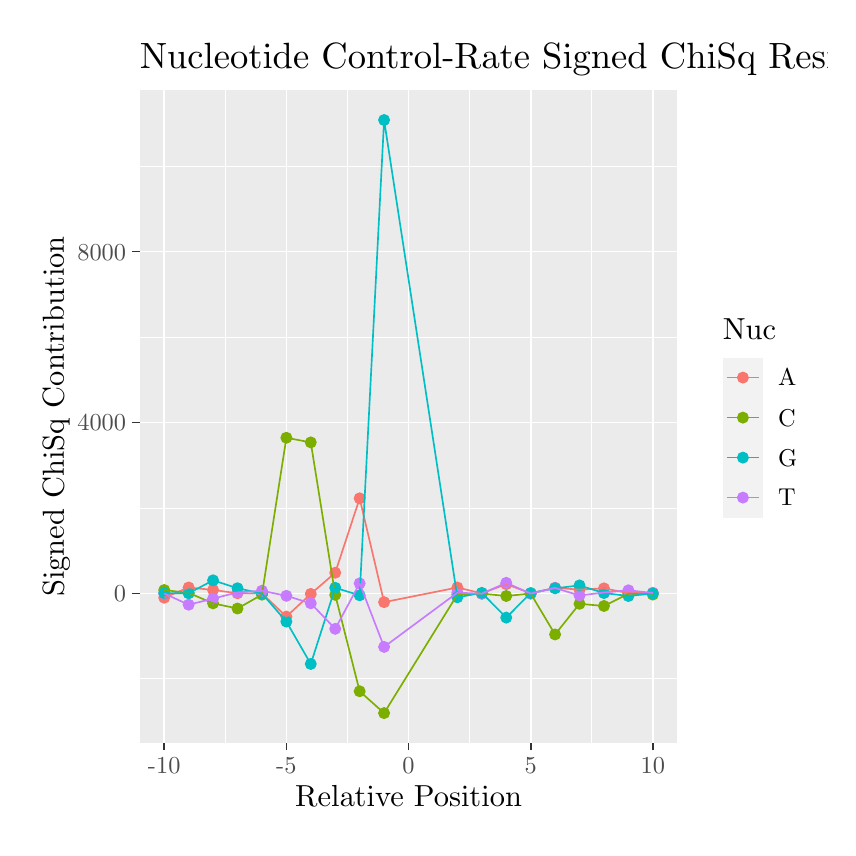
\begin{tikzpicture}[x=1pt,y=1pt]
\definecolor{fillColor}{RGB}{255,255,255}
\path[use as bounding box,fill=fillColor,fill opacity=0.00] (0,0) rectangle (289.08,289.08);
\begin{scope}
\path[clip] (  0.00,  0.00) rectangle (289.08,289.08);
\definecolor{drawColor}{RGB}{255,255,255}
\definecolor{fillColor}{RGB}{255,255,255}

\path[draw=drawColor,line width= 0.6pt,line join=round,line cap=round,fill=fillColor] (  0.00,  0.00) rectangle (289.08,289.08);
\end{scope}
\begin{scope}
\path[clip] ( 40.51, 30.69) rectangle (234.72,266.42);
\definecolor{fillColor}{gray}{0.92}

\path[fill=fillColor] ( 40.51, 30.69) rectangle (234.72,266.42);
\definecolor{drawColor}{RGB}{255,255,255}

\path[draw=drawColor,line width= 0.3pt,line join=round] ( 40.51, 53.78) --
	(234.72, 53.78);

\path[draw=drawColor,line width= 0.3pt,line join=round] ( 40.51,115.53) --
	(234.72,115.53);

\path[draw=drawColor,line width= 0.3pt,line join=round] ( 40.51,177.27) --
	(234.72,177.27);

\path[draw=drawColor,line width= 0.3pt,line join=round] ( 40.51,239.02) --
	(234.72,239.02);

\path[draw=drawColor,line width= 0.3pt,line join=round] ( 71.41, 30.69) --
	( 71.41,266.42);

\path[draw=drawColor,line width= 0.3pt,line join=round] (115.55, 30.69) --
	(115.55,266.42);

\path[draw=drawColor,line width= 0.3pt,line join=round] (159.69, 30.69) --
	(159.69,266.42);

\path[draw=drawColor,line width= 0.3pt,line join=round] (203.82, 30.69) --
	(203.82,266.42);

\path[draw=drawColor,line width= 0.6pt,line join=round] ( 40.51, 84.65) --
	(234.72, 84.65);

\path[draw=drawColor,line width= 0.6pt,line join=round] ( 40.51,146.40) --
	(234.72,146.40);

\path[draw=drawColor,line width= 0.6pt,line join=round] ( 40.51,208.15) --
	(234.72,208.15);

\path[draw=drawColor,line width= 0.6pt,line join=round] ( 49.34, 30.69) --
	( 49.34,266.42);

\path[draw=drawColor,line width= 0.6pt,line join=round] ( 93.48, 30.69) --
	( 93.48,266.42);

\path[draw=drawColor,line width= 0.6pt,line join=round] (137.62, 30.69) --
	(137.62,266.42);

\path[draw=drawColor,line width= 0.6pt,line join=round] (181.76, 30.69) --
	(181.76,266.42);

\path[draw=drawColor,line width= 0.6pt,line join=round] (225.89, 30.69) --
	(225.89,266.42);
\definecolor{drawColor}{RGB}{248,118,109}
\definecolor{fillColor}{RGB}{248,118,109}

\path[draw=drawColor,line width= 0.4pt,line join=round,line cap=round,fill=fillColor] ( 49.34, 83.10) circle (  1.96);
\definecolor{drawColor}{RGB}{124,174,0}
\definecolor{fillColor}{RGB}{124,174,0}

\path[draw=drawColor,line width= 0.4pt,line join=round,line cap=round,fill=fillColor] ( 49.34, 85.87) circle (  1.96);
\definecolor{drawColor}{RGB}{199,124,255}
\definecolor{fillColor}{RGB}{199,124,255}

\path[draw=drawColor,line width= 0.4pt,line join=round,line cap=round,fill=fillColor] ( 49.34, 84.61) circle (  1.96);
\definecolor{drawColor}{RGB}{0,191,196}
\definecolor{fillColor}{RGB}{0,191,196}

\path[draw=drawColor,line width= 0.4pt,line join=round,line cap=round,fill=fillColor] ( 49.34, 84.76) circle (  1.96);
\definecolor{drawColor}{RGB}{248,118,109}
\definecolor{fillColor}{RGB}{248,118,109}

\path[draw=drawColor,line width= 0.4pt,line join=round,line cap=round,fill=fillColor] ( 58.17, 86.79) circle (  1.96);
\definecolor{drawColor}{RGB}{124,174,0}
\definecolor{fillColor}{RGB}{124,174,0}

\path[draw=drawColor,line width= 0.4pt,line join=round,line cap=round,fill=fillColor] ( 58.17, 84.83) circle (  1.96);
\definecolor{drawColor}{RGB}{199,124,255}
\definecolor{fillColor}{RGB}{199,124,255}

\path[draw=drawColor,line width= 0.4pt,line join=round,line cap=round,fill=fillColor] ( 58.17, 80.57) circle (  1.96);
\definecolor{drawColor}{RGB}{0,191,196}
\definecolor{fillColor}{RGB}{0,191,196}

\path[draw=drawColor,line width= 0.4pt,line join=round,line cap=round,fill=fillColor] ( 58.17, 84.69) circle (  1.96);
\definecolor{drawColor}{RGB}{248,118,109}
\definecolor{fillColor}{RGB}{248,118,109}

\path[draw=drawColor,line width= 0.4pt,line join=round,line cap=round,fill=fillColor] ( 66.99, 85.91) circle (  1.96);
\definecolor{drawColor}{RGB}{124,174,0}
\definecolor{fillColor}{RGB}{124,174,0}

\path[draw=drawColor,line width= 0.4pt,line join=round,line cap=round,fill=fillColor] ( 66.99, 81.06) circle (  1.96);
\definecolor{drawColor}{RGB}{199,124,255}
\definecolor{fillColor}{RGB}{199,124,255}

\path[draw=drawColor,line width= 0.4pt,line join=round,line cap=round,fill=fillColor] ( 66.99, 82.75) circle (  1.96);
\definecolor{drawColor}{RGB}{0,191,196}
\definecolor{fillColor}{RGB}{0,191,196}

\path[draw=drawColor,line width= 0.4pt,line join=round,line cap=round,fill=fillColor] ( 66.99, 89.38) circle (  1.96);
\definecolor{drawColor}{RGB}{248,118,109}
\definecolor{fillColor}{RGB}{248,118,109}

\path[draw=drawColor,line width= 0.4pt,line join=round,line cap=round,fill=fillColor] ( 75.82, 84.70) circle (  1.96);
\definecolor{drawColor}{RGB}{124,174,0}
\definecolor{fillColor}{RGB}{124,174,0}

\path[draw=drawColor,line width= 0.4pt,line join=round,line cap=round,fill=fillColor] ( 75.82, 79.19) circle (  1.96);
\definecolor{drawColor}{RGB}{199,124,255}
\definecolor{fillColor}{RGB}{199,124,255}

\path[draw=drawColor,line width= 0.4pt,line join=round,line cap=round,fill=fillColor] ( 75.82, 85.03) circle (  1.96);
\definecolor{drawColor}{RGB}{0,191,196}
\definecolor{fillColor}{RGB}{0,191,196}

\path[draw=drawColor,line width= 0.4pt,line join=round,line cap=round,fill=fillColor] ( 75.82, 86.52) circle (  1.96);
\definecolor{drawColor}{RGB}{248,118,109}
\definecolor{fillColor}{RGB}{248,118,109}

\path[draw=drawColor,line width= 0.4pt,line join=round,line cap=round,fill=fillColor] ( 84.65, 84.64) circle (  1.96);
\definecolor{drawColor}{RGB}{124,174,0}
\definecolor{fillColor}{RGB}{124,174,0}

\path[draw=drawColor,line width= 0.4pt,line join=round,line cap=round,fill=fillColor] ( 84.65, 84.20) circle (  1.96);
\definecolor{drawColor}{RGB}{0,191,196}
\definecolor{fillColor}{RGB}{0,191,196}

\path[draw=drawColor,line width= 0.4pt,line join=round,line cap=round,fill=fillColor] ( 84.65, 84.62) circle (  1.96);
\definecolor{drawColor}{RGB}{199,124,255}
\definecolor{fillColor}{RGB}{199,124,255}

\path[draw=drawColor,line width= 0.4pt,line join=round,line cap=round,fill=fillColor] ( 84.65, 85.62) circle (  1.96);
\definecolor{drawColor}{RGB}{248,118,109}
\definecolor{fillColor}{RGB}{248,118,109}

\path[draw=drawColor,line width= 0.4pt,line join=round,line cap=round,fill=fillColor] ( 93.48, 76.27) circle (  1.96);
\definecolor{drawColor}{RGB}{124,174,0}
\definecolor{fillColor}{RGB}{124,174,0}

\path[draw=drawColor,line width= 0.4pt,line join=round,line cap=round,fill=fillColor] ( 93.48,140.89) circle (  1.96);
\definecolor{drawColor}{RGB}{0,191,196}
\definecolor{fillColor}{RGB}{0,191,196}

\path[draw=drawColor,line width= 0.4pt,line join=round,line cap=round,fill=fillColor] ( 93.48, 74.46) circle (  1.96);
\definecolor{drawColor}{RGB}{199,124,255}
\definecolor{fillColor}{RGB}{199,124,255}

\path[draw=drawColor,line width= 0.4pt,line join=round,line cap=round,fill=fillColor] ( 93.48, 83.78) circle (  1.96);
\definecolor{drawColor}{RGB}{248,118,109}
\definecolor{fillColor}{RGB}{248,118,109}

\path[draw=drawColor,line width= 0.4pt,line join=round,line cap=round,fill=fillColor] (102.30, 84.47) circle (  1.96);
\definecolor{drawColor}{RGB}{124,174,0}
\definecolor{fillColor}{RGB}{124,174,0}

\path[draw=drawColor,line width= 0.4pt,line join=round,line cap=round,fill=fillColor] (102.30,139.22) circle (  1.96);
\definecolor{drawColor}{RGB}{0,191,196}
\definecolor{fillColor}{RGB}{0,191,196}

\path[draw=drawColor,line width= 0.4pt,line join=round,line cap=round,fill=fillColor] (102.30, 59.16) circle (  1.96);
\definecolor{drawColor}{RGB}{199,124,255}
\definecolor{fillColor}{RGB}{199,124,255}

\path[draw=drawColor,line width= 0.4pt,line join=round,line cap=round,fill=fillColor] (102.30, 81.07) circle (  1.96);
\definecolor{drawColor}{RGB}{248,118,109}
\definecolor{fillColor}{RGB}{248,118,109}

\path[draw=drawColor,line width= 0.4pt,line join=round,line cap=round,fill=fillColor] (111.13, 92.11) circle (  1.96);
\definecolor{drawColor}{RGB}{124,174,0}
\definecolor{fillColor}{RGB}{124,174,0}

\path[draw=drawColor,line width= 0.4pt,line join=round,line cap=round,fill=fillColor] (111.13, 84.14) circle (  1.96);
\definecolor{drawColor}{RGB}{199,124,255}
\definecolor{fillColor}{RGB}{199,124,255}

\path[draw=drawColor,line width= 0.4pt,line join=round,line cap=round,fill=fillColor] (111.13, 71.85) circle (  1.96);
\definecolor{drawColor}{RGB}{0,191,196}
\definecolor{fillColor}{RGB}{0,191,196}

\path[draw=drawColor,line width= 0.4pt,line join=round,line cap=round,fill=fillColor] (111.13, 86.68) circle (  1.96);
\definecolor{drawColor}{RGB}{248,118,109}
\definecolor{fillColor}{RGB}{248,118,109}

\path[draw=drawColor,line width= 0.4pt,line join=round,line cap=round,fill=fillColor] (119.96,119.01) circle (  1.96);
\definecolor{drawColor}{RGB}{124,174,0}
\definecolor{fillColor}{RGB}{124,174,0}

\path[draw=drawColor,line width= 0.4pt,line join=round,line cap=round,fill=fillColor] (119.96, 49.29) circle (  1.96);
\definecolor{drawColor}{RGB}{0,191,196}
\definecolor{fillColor}{RGB}{0,191,196}

\path[draw=drawColor,line width= 0.4pt,line join=round,line cap=round,fill=fillColor] (119.96, 83.97) circle (  1.96);
\definecolor{drawColor}{RGB}{199,124,255}
\definecolor{fillColor}{RGB}{199,124,255}

\path[draw=drawColor,line width= 0.4pt,line join=round,line cap=round,fill=fillColor] (119.96, 88.27) circle (  1.96);
\definecolor{drawColor}{RGB}{248,118,109}
\definecolor{fillColor}{RGB}{248,118,109}

\path[draw=drawColor,line width= 0.4pt,line join=round,line cap=round,fill=fillColor] (128.79, 81.49) circle (  1.96);
\definecolor{drawColor}{RGB}{124,174,0}
\definecolor{fillColor}{RGB}{124,174,0}

\path[draw=drawColor,line width= 0.4pt,line join=round,line cap=round,fill=fillColor] (128.79, 41.40) circle (  1.96);
\definecolor{drawColor}{RGB}{0,191,196}
\definecolor{fillColor}{RGB}{0,191,196}

\path[draw=drawColor,line width= 0.4pt,line join=round,line cap=round,fill=fillColor] (128.79,255.71) circle (  1.96);
\definecolor{drawColor}{RGB}{199,124,255}
\definecolor{fillColor}{RGB}{199,124,255}

\path[draw=drawColor,line width= 0.4pt,line join=round,line cap=round,fill=fillColor] (128.79, 65.32) circle (  1.96);
\definecolor{drawColor}{RGB}{248,118,109}
\definecolor{fillColor}{RGB}{248,118,109}

\path[draw=drawColor,line width= 0.4pt,line join=round,line cap=round,fill=fillColor] (155.27, 86.78) circle (  1.96);
\definecolor{drawColor}{RGB}{124,174,0}
\definecolor{fillColor}{RGB}{124,174,0}

\path[draw=drawColor,line width= 0.4pt,line join=round,line cap=round,fill=fillColor] (155.27, 84.23) circle (  1.96);
\definecolor{drawColor}{RGB}{199,124,255}
\definecolor{fillColor}{RGB}{199,124,255}

\path[draw=drawColor,line width= 0.4pt,line join=round,line cap=round,fill=fillColor] (155.27, 84.92) circle (  1.96);
\definecolor{drawColor}{RGB}{0,191,196}
\definecolor{fillColor}{RGB}{0,191,196}

\path[draw=drawColor,line width= 0.4pt,line join=round,line cap=round,fill=fillColor] (155.27, 83.24) circle (  1.96);
\definecolor{drawColor}{RGB}{248,118,109}
\definecolor{fillColor}{RGB}{248,118,109}

\path[draw=drawColor,line width= 0.4pt,line join=round,line cap=round,fill=fillColor] (164.10, 84.67) circle (  1.96);
\definecolor{drawColor}{RGB}{124,174,0}
\definecolor{fillColor}{RGB}{124,174,0}

\path[draw=drawColor,line width= 0.4pt,line join=round,line cap=round,fill=fillColor] (164.10, 84.58) circle (  1.96);
\definecolor{drawColor}{RGB}{199,124,255}
\definecolor{fillColor}{RGB}{199,124,255}

\path[draw=drawColor,line width= 0.4pt,line join=round,line cap=round,fill=fillColor] (164.10, 84.54) circle (  1.96);
\definecolor{drawColor}{RGB}{0,191,196}
\definecolor{fillColor}{RGB}{0,191,196}

\path[draw=drawColor,line width= 0.4pt,line join=round,line cap=round,fill=fillColor] (164.10, 84.84) circle (  1.96);
\definecolor{drawColor}{RGB}{248,118,109}
\definecolor{fillColor}{RGB}{248,118,109}

\path[draw=drawColor,line width= 0.4pt,line join=round,line cap=round,fill=fillColor] (172.93, 88.00) circle (  1.96);
\definecolor{drawColor}{RGB}{124,174,0}
\definecolor{fillColor}{RGB}{124,174,0}

\path[draw=drawColor,line width= 0.4pt,line join=round,line cap=round,fill=fillColor] (172.93, 83.71) circle (  1.96);
\definecolor{drawColor}{RGB}{199,124,255}
\definecolor{fillColor}{RGB}{199,124,255}

\path[draw=drawColor,line width= 0.4pt,line join=round,line cap=round,fill=fillColor] (172.93, 88.47) circle (  1.96);
\definecolor{drawColor}{RGB}{0,191,196}
\definecolor{fillColor}{RGB}{0,191,196}

\path[draw=drawColor,line width= 0.4pt,line join=round,line cap=round,fill=fillColor] (172.93, 75.91) circle (  1.96);
\definecolor{drawColor}{RGB}{248,118,109}
\definecolor{fillColor}{RGB}{248,118,109}

\path[draw=drawColor,line width= 0.4pt,line join=round,line cap=round,fill=fillColor] (181.76, 84.69) circle (  1.96);
\definecolor{drawColor}{RGB}{124,174,0}
\definecolor{fillColor}{RGB}{124,174,0}

\path[draw=drawColor,line width= 0.4pt,line join=round,line cap=round,fill=fillColor] (181.76, 84.60) circle (  1.96);
\definecolor{drawColor}{RGB}{199,124,255}
\definecolor{fillColor}{RGB}{199,124,255}

\path[draw=drawColor,line width= 0.4pt,line join=round,line cap=round,fill=fillColor] (181.76, 84.59) circle (  1.96);
\definecolor{drawColor}{RGB}{0,191,196}
\definecolor{fillColor}{RGB}{0,191,196}

\path[draw=drawColor,line width= 0.4pt,line join=round,line cap=round,fill=fillColor] (181.76, 84.76) circle (  1.96);
\definecolor{drawColor}{RGB}{248,118,109}
\definecolor{fillColor}{RGB}{248,118,109}

\path[draw=drawColor,line width= 0.4pt,line join=round,line cap=round,fill=fillColor] (190.58, 86.68) circle (  1.96);
\definecolor{drawColor}{RGB}{124,174,0}
\definecolor{fillColor}{RGB}{124,174,0}

\path[draw=drawColor,line width= 0.4pt,line join=round,line cap=round,fill=fillColor] (190.58, 69.82) circle (  1.96);
\definecolor{drawColor}{RGB}{199,124,255}
\definecolor{fillColor}{RGB}{199,124,255}

\path[draw=drawColor,line width= 0.4pt,line join=round,line cap=round,fill=fillColor] (190.58, 86.61) circle (  1.96);
\definecolor{drawColor}{RGB}{0,191,196}
\definecolor{fillColor}{RGB}{0,191,196}

\path[draw=drawColor,line width= 0.4pt,line join=round,line cap=round,fill=fillColor] (190.58, 86.49) circle (  1.96);
\definecolor{drawColor}{RGB}{248,118,109}
\definecolor{fillColor}{RGB}{248,118,109}

\path[draw=drawColor,line width= 0.4pt,line join=round,line cap=round,fill=fillColor] (199.41, 86.02) circle (  1.96);
\definecolor{drawColor}{RGB}{124,174,0}
\definecolor{fillColor}{RGB}{124,174,0}

\path[draw=drawColor,line width= 0.4pt,line join=round,line cap=round,fill=fillColor] (199.41, 80.89) circle (  1.96);
\definecolor{drawColor}{RGB}{199,124,255}
\definecolor{fillColor}{RGB}{199,124,255}

\path[draw=drawColor,line width= 0.4pt,line join=round,line cap=round,fill=fillColor] (199.41, 83.90) circle (  1.96);
\definecolor{drawColor}{RGB}{0,191,196}
\definecolor{fillColor}{RGB}{0,191,196}

\path[draw=drawColor,line width= 0.4pt,line join=round,line cap=round,fill=fillColor] (199.41, 87.54) circle (  1.96);
\definecolor{drawColor}{RGB}{248,118,109}
\definecolor{fillColor}{RGB}{248,118,109}

\path[draw=drawColor,line width= 0.4pt,line join=round,line cap=round,fill=fillColor] (208.24, 86.48) circle (  1.96);
\definecolor{drawColor}{RGB}{124,174,0}
\definecolor{fillColor}{RGB}{124,174,0}

\path[draw=drawColor,line width= 0.4pt,line join=round,line cap=round,fill=fillColor] (208.24, 80.11) circle (  1.96);
\definecolor{drawColor}{RGB}{199,124,255}
\definecolor{fillColor}{RGB}{199,124,255}

\path[draw=drawColor,line width= 0.4pt,line join=round,line cap=round,fill=fillColor] (208.24, 84.98) circle (  1.96);
\definecolor{drawColor}{RGB}{0,191,196}
\definecolor{fillColor}{RGB}{0,191,196}

\path[draw=drawColor,line width= 0.4pt,line join=round,line cap=round,fill=fillColor] (208.24, 84.78) circle (  1.96);
\definecolor{drawColor}{RGB}{248,118,109}
\definecolor{fillColor}{RGB}{248,118,109}

\path[draw=drawColor,line width= 0.4pt,line join=round,line cap=round,fill=fillColor] (217.07, 84.75) circle (  1.96);
\definecolor{drawColor}{RGB}{124,174,0}
\definecolor{fillColor}{RGB}{124,174,0}

\path[draw=drawColor,line width= 0.4pt,line join=round,line cap=round,fill=fillColor] (217.07, 84.52) circle (  1.96);
\definecolor{drawColor}{RGB}{0,191,196}
\definecolor{fillColor}{RGB}{0,191,196}

\path[draw=drawColor,line width= 0.4pt,line join=round,line cap=round,fill=fillColor] (217.07, 83.71) circle (  1.96);
\definecolor{drawColor}{RGB}{199,124,255}
\definecolor{fillColor}{RGB}{199,124,255}

\path[draw=drawColor,line width= 0.4pt,line join=round,line cap=round,fill=fillColor] (217.07, 85.78) circle (  1.96);
\definecolor{drawColor}{RGB}{248,118,109}
\definecolor{fillColor}{RGB}{248,118,109}

\path[draw=drawColor,line width= 0.4pt,line join=round,line cap=round,fill=fillColor] (225.89, 84.84) circle (  1.96);
\definecolor{drawColor}{RGB}{124,174,0}
\definecolor{fillColor}{RGB}{124,174,0}

\path[draw=drawColor,line width= 0.4pt,line join=round,line cap=round,fill=fillColor] (225.89, 84.22) circle (  1.96);
\definecolor{drawColor}{RGB}{199,124,255}
\definecolor{fillColor}{RGB}{199,124,255}

\path[draw=drawColor,line width= 0.4pt,line join=round,line cap=round,fill=fillColor] (225.89, 84.81) circle (  1.96);
\definecolor{drawColor}{RGB}{0,191,196}
\definecolor{fillColor}{RGB}{0,191,196}

\path[draw=drawColor,line width= 0.4pt,line join=round,line cap=round,fill=fillColor] (225.89, 84.63) circle (  1.96);
\definecolor{drawColor}{RGB}{248,118,109}

\path[draw=drawColor,line width= 0.6pt,line join=round] ( 49.34, 83.10) --
	( 58.17, 86.79) --
	( 66.99, 85.91) --
	( 75.82, 84.70) --
	( 84.65, 84.64) --
	( 93.48, 76.27) --
	(102.30, 84.47) --
	(111.13, 92.11) --
	(119.96,119.01) --
	(128.79, 81.49) --
	(155.27, 86.78) --
	(164.10, 84.67) --
	(172.93, 88.00) --
	(181.76, 84.69) --
	(190.58, 86.68) --
	(199.41, 86.02) --
	(208.24, 86.48) --
	(217.07, 84.75) --
	(225.89, 84.84);
\definecolor{drawColor}{RGB}{124,174,0}

\path[draw=drawColor,line width= 0.6pt,line join=round] ( 49.34, 85.87) --
	( 58.17, 84.83) --
	( 66.99, 81.06) --
	( 75.82, 79.19) --
	( 84.65, 84.20) --
	( 93.48,140.89) --
	(102.30,139.22) --
	(111.13, 84.14) --
	(119.96, 49.29) --
	(128.79, 41.40) --
	(155.27, 84.23) --
	(164.10, 84.58) --
	(172.93, 83.71) --
	(181.76, 84.60) --
	(190.58, 69.82) --
	(199.41, 80.89) --
	(208.24, 80.11) --
	(217.07, 84.52) --
	(225.89, 84.22);
\definecolor{drawColor}{RGB}{0,191,196}

\path[draw=drawColor,line width= 0.6pt,line join=round] ( 49.34, 84.76) --
	( 58.17, 84.69) --
	( 66.99, 89.38) --
	( 75.82, 86.52) --
	( 84.65, 84.62) --
	( 93.48, 74.46) --
	(102.30, 59.16) --
	(111.13, 86.68) --
	(119.96, 83.97) --
	(128.79,255.71) --
	(155.27, 83.24) --
	(164.10, 84.84) --
	(172.93, 75.91) --
	(181.76, 84.76) --
	(190.58, 86.49) --
	(199.41, 87.54) --
	(208.24, 84.78) --
	(217.07, 83.71) --
	(225.89, 84.63);
\definecolor{drawColor}{RGB}{199,124,255}

\path[draw=drawColor,line width= 0.6pt,line join=round] ( 49.34, 84.61) --
	( 58.17, 80.57) --
	( 66.99, 82.75) --
	( 75.82, 85.03) --
	( 84.65, 85.62) --
	( 93.48, 83.78) --
	(102.30, 81.07) --
	(111.13, 71.85) --
	(119.96, 88.27) --
	(128.79, 65.32) --
	(155.27, 84.92) --
	(164.10, 84.54) --
	(172.93, 88.47) --
	(181.76, 84.59) --
	(190.58, 86.61) --
	(199.41, 83.90) --
	(208.24, 84.98) --
	(217.07, 85.78) --
	(225.89, 84.81);
\end{scope}
\begin{scope}
\path[clip] (  0.00,  0.00) rectangle (289.08,289.08);
\definecolor{drawColor}{gray}{0.30}

\node[text=drawColor,anchor=base east,inner sep=0pt, outer sep=0pt, scale=  0.88] at ( 35.56, 81.62) {0};

\node[text=drawColor,anchor=base east,inner sep=0pt, outer sep=0pt, scale=  0.88] at ( 35.56,143.37) {4000};

\node[text=drawColor,anchor=base east,inner sep=0pt, outer sep=0pt, scale=  0.88] at ( 35.56,205.12) {8000};
\end{scope}
\begin{scope}
\path[clip] (  0.00,  0.00) rectangle (289.08,289.08);
\definecolor{drawColor}{gray}{0.20}

\path[draw=drawColor,line width= 0.6pt,line join=round] ( 37.76, 84.65) --
	( 40.51, 84.65);

\path[draw=drawColor,line width= 0.6pt,line join=round] ( 37.76,146.40) --
	( 40.51,146.40);

\path[draw=drawColor,line width= 0.6pt,line join=round] ( 37.76,208.15) --
	( 40.51,208.15);
\end{scope}
\begin{scope}
\path[clip] (  0.00,  0.00) rectangle (289.08,289.08);
\definecolor{drawColor}{gray}{0.20}

\path[draw=drawColor,line width= 0.6pt,line join=round] ( 49.34, 27.94) --
	( 49.34, 30.69);

\path[draw=drawColor,line width= 0.6pt,line join=round] ( 93.48, 27.94) --
	( 93.48, 30.69);

\path[draw=drawColor,line width= 0.6pt,line join=round] (137.62, 27.94) --
	(137.62, 30.69);

\path[draw=drawColor,line width= 0.6pt,line join=round] (181.76, 27.94) --
	(181.76, 30.69);

\path[draw=drawColor,line width= 0.6pt,line join=round] (225.89, 27.94) --
	(225.89, 30.69);
\end{scope}
\begin{scope}
\path[clip] (  0.00,  0.00) rectangle (289.08,289.08);
\definecolor{drawColor}{gray}{0.30}

\node[text=drawColor,anchor=base,inner sep=0pt, outer sep=0pt, scale=  0.88] at ( 49.34, 19.68) {-10};

\node[text=drawColor,anchor=base,inner sep=0pt, outer sep=0pt, scale=  0.88] at ( 93.48, 19.68) {-5};

\node[text=drawColor,anchor=base,inner sep=0pt, outer sep=0pt, scale=  0.88] at (137.62, 19.68) {0};

\node[text=drawColor,anchor=base,inner sep=0pt, outer sep=0pt, scale=  0.88] at (181.76, 19.68) {5};

\node[text=drawColor,anchor=base,inner sep=0pt, outer sep=0pt, scale=  0.88] at (225.89, 19.68) {10};
\end{scope}
\begin{scope}
\path[clip] (  0.00,  0.00) rectangle (289.08,289.08);
\definecolor{drawColor}{RGB}{0,0,0}

\node[text=drawColor,anchor=base,inner sep=0pt, outer sep=0pt, scale=  1.10] at (137.62,  7.64) {Relative Position};
\end{scope}
\begin{scope}
\path[clip] (  0.00,  0.00) rectangle (289.08,289.08);
\definecolor{drawColor}{RGB}{0,0,0}

\node[text=drawColor,rotate= 90.00,anchor=base,inner sep=0pt, outer sep=0pt, scale=  1.10] at ( 13.08,148.55) {Signed ChiSq Contribution};
\end{scope}
\begin{scope}
\path[clip] (  0.00,  0.00) rectangle (289.08,289.08);
\definecolor{fillColor}{RGB}{255,255,255}

\path[fill=fillColor] (245.72,106.54) rectangle (283.58,190.57);
\end{scope}
\begin{scope}
\path[clip] (  0.00,  0.00) rectangle (289.08,289.08);
\definecolor{drawColor}{RGB}{0,0,0}

\node[text=drawColor,anchor=base west,inner sep=0pt, outer sep=0pt, scale=  1.10] at (251.22,176.42) {Nuc};
\end{scope}
\begin{scope}
\path[clip] (  0.00,  0.00) rectangle (289.08,289.08);
\definecolor{fillColor}{gray}{0.95}

\path[fill=fillColor] (251.22,155.40) rectangle (265.68,169.86);
\end{scope}
\begin{scope}
\path[clip] (  0.00,  0.00) rectangle (289.08,289.08);
\definecolor{drawColor}{RGB}{248,118,109}
\definecolor{fillColor}{RGB}{248,118,109}

\path[draw=drawColor,line width= 0.4pt,line join=round,line cap=round,fill=fillColor] (258.45,162.63) circle (  1.96);
\end{scope}
\begin{scope}
\path[clip] (  0.00,  0.00) rectangle (289.08,289.08);
\definecolor{drawColor}{RGB}{248,118,109}

\path[draw=drawColor,line width= 0.6pt,line join=round] (252.67,162.63) -- (264.23,162.63);
\end{scope}
\begin{scope}
\path[clip] (  0.00,  0.00) rectangle (289.08,289.08);
\definecolor{fillColor}{gray}{0.95}

\path[fill=fillColor] (251.22,140.95) rectangle (265.68,155.40);
\end{scope}
\begin{scope}
\path[clip] (  0.00,  0.00) rectangle (289.08,289.08);
\definecolor{drawColor}{RGB}{124,174,0}
\definecolor{fillColor}{RGB}{124,174,0}

\path[draw=drawColor,line width= 0.4pt,line join=round,line cap=round,fill=fillColor] (258.45,148.17) circle (  1.96);
\end{scope}
\begin{scope}
\path[clip] (  0.00,  0.00) rectangle (289.08,289.08);
\definecolor{drawColor}{RGB}{124,174,0}

\path[draw=drawColor,line width= 0.6pt,line join=round] (252.67,148.17) -- (264.23,148.17);
\end{scope}
\begin{scope}
\path[clip] (  0.00,  0.00) rectangle (289.08,289.08);
\definecolor{fillColor}{gray}{0.95}

\path[fill=fillColor] (251.22,126.49) rectangle (265.68,140.95);
\end{scope}
\begin{scope}
\path[clip] (  0.00,  0.00) rectangle (289.08,289.08);
\definecolor{drawColor}{RGB}{0,191,196}
\definecolor{fillColor}{RGB}{0,191,196}

\path[draw=drawColor,line width= 0.4pt,line join=round,line cap=round,fill=fillColor] (258.45,133.72) circle (  1.96);
\end{scope}
\begin{scope}
\path[clip] (  0.00,  0.00) rectangle (289.08,289.08);
\definecolor{drawColor}{RGB}{0,191,196}

\path[draw=drawColor,line width= 0.6pt,line join=round] (252.67,133.72) -- (264.23,133.72);
\end{scope}
\begin{scope}
\path[clip] (  0.00,  0.00) rectangle (289.08,289.08);
\definecolor{fillColor}{gray}{0.95}

\path[fill=fillColor] (251.22,112.04) rectangle (265.68,126.49);
\end{scope}
\begin{scope}
\path[clip] (  0.00,  0.00) rectangle (289.08,289.08);
\definecolor{drawColor}{RGB}{199,124,255}
\definecolor{fillColor}{RGB}{199,124,255}

\path[draw=drawColor,line width= 0.4pt,line join=round,line cap=round,fill=fillColor] (258.45,119.27) circle (  1.96);
\end{scope}
\begin{scope}
\path[clip] (  0.00,  0.00) rectangle (289.08,289.08);
\definecolor{drawColor}{RGB}{199,124,255}

\path[draw=drawColor,line width= 0.6pt,line join=round] (252.67,119.27) -- (264.23,119.27);
\end{scope}
\begin{scope}
\path[clip] (  0.00,  0.00) rectangle (289.08,289.08);
\definecolor{drawColor}{RGB}{0,0,0}

\node[text=drawColor,anchor=base west,inner sep=0pt, outer sep=0pt, scale=  0.88] at (271.18,159.60) {A};
\end{scope}
\begin{scope}
\path[clip] (  0.00,  0.00) rectangle (289.08,289.08);
\definecolor{drawColor}{RGB}{0,0,0}

\node[text=drawColor,anchor=base west,inner sep=0pt, outer sep=0pt, scale=  0.88] at (271.18,145.14) {C};
\end{scope}
\begin{scope}
\path[clip] (  0.00,  0.00) rectangle (289.08,289.08);
\definecolor{drawColor}{RGB}{0,0,0}

\node[text=drawColor,anchor=base west,inner sep=0pt, outer sep=0pt, scale=  0.88] at (271.18,130.69) {G};
\end{scope}
\begin{scope}
\path[clip] (  0.00,  0.00) rectangle (289.08,289.08);
\definecolor{drawColor}{RGB}{0,0,0}

\node[text=drawColor,anchor=base west,inner sep=0pt, outer sep=0pt, scale=  0.88] at (271.18,116.24) {T};
\end{scope}
\begin{scope}
\path[clip] (  0.00,  0.00) rectangle (289.08,289.08);
\definecolor{drawColor}{RGB}{0,0,0}

\node[text=drawColor,anchor=base west,inner sep=0pt, outer sep=0pt, scale=  1.32] at ( 40.51,274.49) {Nucleotide Control-Rate Signed ChiSq Residual: cpg-GC-TA};
\end{scope}
\end{tikzpicture}
